\documentclass[12pt]{article}

\usepackage{amsmath}
\usepackage{amsthm}
\usepackage{float}
\usepackage{graphicx}
\usepackage{tikz}

\title{EECS 440 HW6}
\author{Andrew Mason}

\begin{document}
\maketitle

\begin{enumerate}
  \item
    % 1
    \begin{enumerate}
      \item
        We can construct another network by inserting ``dummy'' nodes, which
        will serve to place the hidden nodes that were in the same layer in
        different layers in the constructed network.\\
        For example:
        \begin{center}
          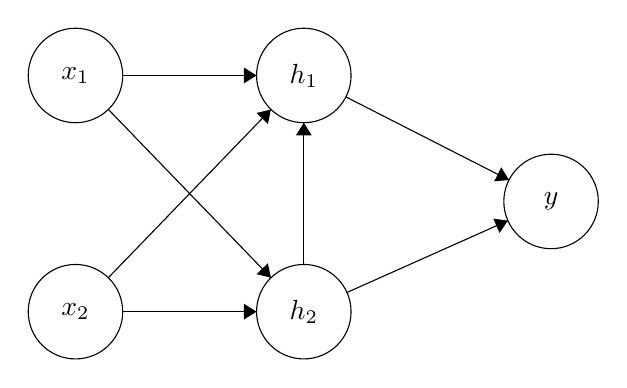
\begin{tikzpicture}[scale=0.2]
          \tikzstyle{every node}+=[inner sep=0pt]
          \draw [black] (13,-10.7) circle (3);
          \draw (13,-10.7) node {$x_1$};
          \draw [black] (13,-25.7) circle (3);
          \draw (13,-25.7) node {$x_2$};
          \draw [black] (27.5,-10.7) circle (3);
          \draw (27.5,-10.7) node {$h_1$};
          \draw [black] (27.5,-25.7) circle (3);
          \draw (27.5,-25.7) node {$h_2$};
          \draw [black] (43.2,-18.7) circle (3);
          \draw (43.2,-18.7) node {$y$};
          \draw [black] (16,-10.7) -- (24.5,-10.7);
          \fill [black] (24.5,-10.7) -- (23.7,-10.2) -- (23.7,-11.2);
          \draw [black] (15.09,-23.54) -- (25.41,-12.86);
          \fill [black] (25.41,-12.86) -- (24.5,-13.08) -- (25.22,-13.78);
          \draw [black] (15.09,-12.86) -- (25.41,-23.54);
          \fill [black] (25.41,-23.54) -- (25.22,-22.62) -- (24.5,-23.32);
          \draw [black] (16,-25.7) -- (24.5,-25.7);
          \fill [black] (24.5,-25.7) -- (23.7,-25.2) -- (23.7,-26.2);
          \draw [black] (30.17,-12.06) -- (40.53,-17.34);
          \fill [black] (40.53,-17.34) -- (40.04,-16.53) -- (39.59,-17.42);
          \draw [black] (30.24,-24.48) -- (40.46,-19.92);
          \fill [black] (40.46,-19.92) -- (39.53,-19.79) -- (39.93,-20.7);
          \draw [black] (27.5,-22.7) -- (27.5,-13.7);
          \fill [black] (27.5,-13.7) -- (27,-14.5) -- (28,-14.5);
          \end{tikzpicture}
        \end{center}
        Then the constructed network would be:
        \begin{center}
          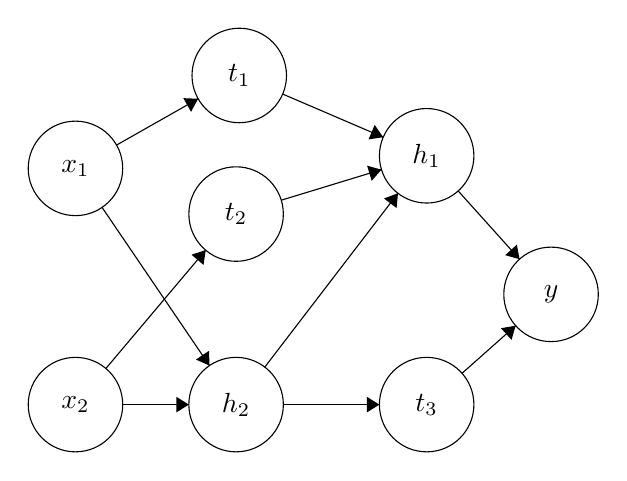
\begin{tikzpicture}[scale=0.2]
          \tikzstyle{every node}+=[inner sep=0pt]
          \draw [black] (13,-10.7) circle (3);
          \draw (13,-10.7) node {$x_1$};
          \draw [black] (13,-25.7) circle (3);
          \draw (13,-25.7) node {$x_2$};
          \draw [black] (35.3,-9.9) circle (3);
          \draw (35.3,-9.9) node {$h_1$};
          \draw [black] (23.2,-25.7) circle (3);
          \draw (23.2,-25.7) node {$h_2$};
          \draw [black] (43.2,-18.7) circle (3);
          \draw (43.2,-18.7) node {$y$};
          \draw [black] (23.4,-4.8) circle (3);
          \draw (23.4,-4.8) node {$t_1$};
          \draw [black] (23.2,-13.6) circle (3);
          \draw (23.2,-13.6) node {$t_2$};
          \draw [black] (35.3,-25.7) circle (3);
          \draw (35.3,-25.7) node {$t_3$};
          \draw [black] (14.69,-13.18) -- (21.51,-23.22);
          \fill [black] (21.51,-23.22) -- (21.48,-22.28) -- (20.65,-22.84);
          \draw [black] (16,-25.7) -- (20.2,-25.7);
          \fill [black] (20.2,-25.7) -- (19.4,-25.2) -- (19.4,-26.2);
          \draw [black] (37.3,-12.13) -- (41.2,-16.47);
          \fill [black] (41.2,-16.47) -- (41.03,-15.54) -- (40.29,-16.21);
          \draw [black] (25.02,-23.32) -- (33.48,-12.28);
          \fill [black] (33.48,-12.28) -- (32.59,-12.61) -- (33.39,-13.22);
          \draw [black] (15.61,-9.22) -- (20.79,-6.28);
          \fill [black] (20.79,-6.28) -- (19.85,-6.24) -- (20.34,-7.11);
          \draw [black] (26.16,-5.98) -- (32.54,-8.72);
          \fill [black] (32.54,-8.72) -- (32,-7.94) -- (31.61,-8.86);
          \draw [black] (14.93,-23.41) -- (21.27,-15.89);
          \fill [black] (21.27,-15.89) -- (20.37,-16.18) -- (21.13,-16.83);
          \draw [black] (26.07,-12.72) -- (32.43,-10.78);
          \fill [black] (32.43,-10.78) -- (31.52,-10.53) -- (31.81,-11.49);
          \draw [black] (26.2,-25.7) -- (32.3,-25.7);
          \fill [black] (32.3,-25.7) -- (31.5,-25.2) -- (31.5,-26.2);
          \draw [black] (37.55,-23.71) -- (40.95,-20.69);
          \fill [black] (40.95,-20.69) -- (40.02,-20.85) -- (40.69,-21.59);
          \end{tikzpicture}
        \end{center}
        where $t_1, t_2, t_3$ are the dummy nodes which just forward their
        single input onward. Now, this is a feed-forward network, so we can do
        backpropagation as normal.\\
      \item
        This type of network sort of captures a temporal quality of the input
        data, so we can create a similar network which sort of ``unfolds'' the
        network across the time component. The two caveats to this approach is
        we must choose an initial value for the loop, and we can only unfold
        the loop up to a fixed $k$ times (whereas the loop is actually
        infinite). Regardless, this is now a feed-forward network, so we can
        do backpropagation as normal.\\
    \end{enumerate}
  \item
    % 2
    \begin{proof} A neural network with a single hidden layer and a single
      output unit all with sigmoid activation is equivalent to a network where
      the hidden unit activations are $\tanh$ functions, and the ouput unit
      still has a sigmoid activation.\\

      \begin{equation}
        \begin{split}
          \tanh(w,x,a,b)&=a\frac{e^{b\boldsymbol{w}\cdot \boldsymbol{x}}-
                                 e^{-b\boldsymbol{w}\cdot\boldsymbol{x}}}
                                {e^{b\boldsymbol{w}\cdot\boldsymbol{x}}+
                                 e^{-b\boldsymbol{w}\cdot\boldsymbol{x}}}\\
          &=a\frac{\frac{e^{2b\boldsymbol{w}\cdot \boldsymbol{x}}-1}
                   {e^{b\boldsymbol{w}\cdot\boldsymbol{x}}}}
                  {\frac{e^{2b\boldsymbol{w}\cdot\boldsymbol{x}}+1}
                   {e^{b\boldsymbol{w}\cdot\boldsymbol{x}}}}\\
          &=a\frac{e^{2b\boldsymbol{w}\cdot \boldsymbol{x}}-1}
                  {e^{2b\boldsymbol{w}\cdot\boldsymbol{x}}+1}\\
          &=a\left(1-\frac{2}
                         {e^{2b\boldsymbol{w}\cdot\boldsymbol{x}}+1}\right)\\
          \tanh(w,x,-2,-\frac{1}{2})&=
            \frac{2}
                 {e^{-\boldsymbol{w}\cdot\boldsymbol{x}}+1}-1\\
        \end{split}
      \end{equation}

      This expression is $2\times\text{sigmoid}(w,x)-1$. Which means the range
      of the function is (-1,1), whereas the range of the sigmoid function is
      (0,1). At this point, all we need is a function which maps from the range
      (-1,1) to the range (0,1); this defines the weights needed for the output
      unit. This is easy to do, since we can just map the values below zero to
      the range (0, 0.5), and the values $\geq0$ to the range
      $\left[0.5, 1\right)$, using the function $f(x)=\frac{x+1}{2}$.\\
    \end{proof}
  \item
    % 3
    We need an output layer that fires whenever $-7\leq x_1+x_2\leq7$.\\
    \begin{center}
      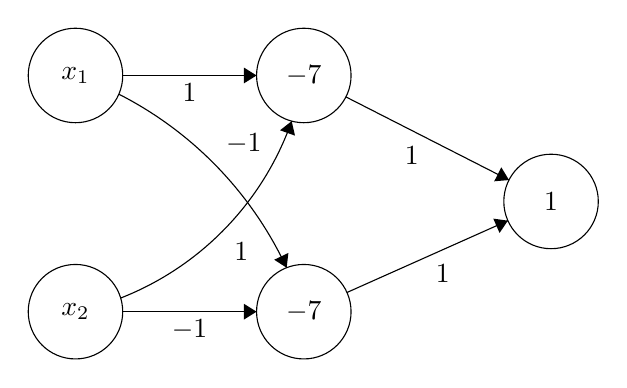
\begin{tikzpicture}[scale=0.2]
      \tikzstyle{every node}+=[inner sep=0pt]
      \draw [black] (13,-10.7) circle (3);
      \draw (13,-10.7) node {$x_1$};
      \draw [black] (13,-25.7) circle (3);
      \draw (13,-25.7) node {$x_2$};
      \draw [black] (27.5,-10.7) circle (3);
      \draw (27.5,-10.7) node {$-7$};
      \draw [black] (27.5,-25.7) circle (3);
      \draw (27.5,-25.7) node {$-7$};
      \draw [black] (43.2,-18.7) circle (3);
      \draw (43.2,-18.7) node {$1$};
      \draw [black] (16,-10.7) -- (24.5,-10.7);
      \fill [black] (24.5,-10.7) -- (23.7,-10.2) -- (23.7,-11.2);
      \draw (20.25,-11.2) node [below] {$1$};
      \draw [black] (26.731,-13.597) arc (-19.44059:-68.61736:18.78);
      \fill [black] (26.73,-13.6) -- (25.99,-14.18) -- (26.94,-14.52);
      \draw (23.05,-21.87) node [right] {$1$};
      \draw [black] (15.753,-11.887) arc (63.02359:25.03436:23.548);
      \fill [black] (26.41,-22.91) -- (26.52,-21.97) -- (25.62,-22.4);
      \draw (22.53,-15.04) node [right] {$-1$};
      \draw [black] (16,-25.7) -- (24.5,-25.7);
      \fill [black] (24.5,-25.7) -- (23.7,-25.2) -- (23.7,-26.2);
      \draw (20.25,-26.2) node [below] {$-1$};
      \draw [black] (30.17,-12.06) -- (40.53,-17.34);
      \fill [black] (40.53,-17.34) -- (40.04,-16.53) -- (39.59,-17.42);
      \draw (34.36,-15.2) node [below] {$1$};
      \draw [black] (30.24,-24.48) -- (40.46,-19.92);
      \fill [black] (40.46,-19.92) -- (39.53,-19.79) -- (39.93,-20.7);
      \draw (36.33,-22.71) node [below] {$1$};
      \end{tikzpicture}
    \end{center}
    Let the upper hidden layer node be $h_1$, the lower hidden layer node be
    $h_2$, and the output node be $y$. Now let`s trace the examples.\\
    \begin{enumerate}
      \item $x_1,x_2,y=-4,-4,-1$\\
        \begin{equation}
          \begin{split}
            h_1&=sign(-8+7)=-1\\
            h_2&=sign(8+7)=1\\
            y&=sign(0-1)=-1\\
          \end{split}
        \end{equation}
      \item $x_1,x_2,y=-1,-1,1$\\
        \begin{equation}
          \begin{split}
            h_1&=sign(-2+7)=1\\
            h_2&=sign(2+7)=1\\
            y&=sign(2-1)=1\\
          \end{split}
        \end{equation}
      \item $x_1,x_2,y=1,1,1$\\
        \begin{equation}
          \begin{split}
            h_1&=sign(2+7)=1\\
            h_2&=sign(-2+7)=1\\
            y&=sign(2-1)=1\\
          \end{split}
        \end{equation}
      \item $x_1,x_2,y=4,4,-1$\\
        \begin{equation}
          \begin{split}
            h_1&=sign(8+7)=1\\
            h_2&=sign(-8+7)=-1\\
            y&=sign(0-1)=-1\\
          \end{split}
        \end{equation}
    \end{enumerate}
  \item
    % 4
    \begin{enumerate}
      \item
        Generated from ``boundaries.py''.
        \begin{figure}[H]
          \includegraphics[width=\linewidth]{neg_10_10.png}
        \end{figure}
      \item
        Generated from ``boundaries.py''.
        \begin{figure}[H]
          \includegraphics[width=\linewidth]{neg_3_3.png}
        \end{figure}
      \item
        Generated from ``boundaries.py''.
        \begin{figure}[H]
          \includegraphics[width=\linewidth]{neg_01_01.png}
        \end{figure}
    \end{enumerate}

    When the weights are given more freedom to range over, the resulting
    ANN can fit the data better - which is shown by the $\left[-10,10\right)$
    graph having a more even positive negative split, as opposed to the
    strictly negative graph for part c.
  \item
    % 5
    You cannot do this for an arbitrary ANN, because it could alter the final
    output of the ANN. Consider the following:
    \begin{center}
      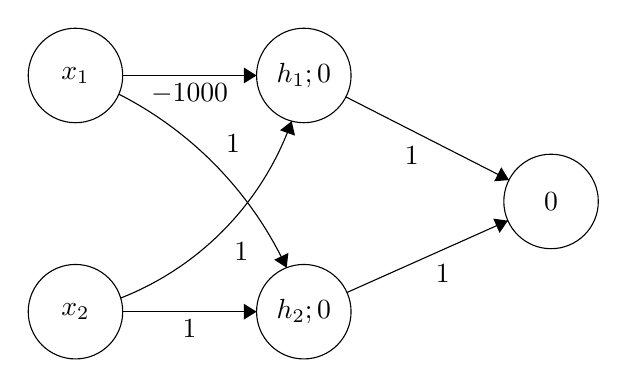
\begin{tikzpicture}[scale=0.2]
      \tikzstyle{every node}+=[inner sep=0pt]
      \draw [black] (13,-10.7) circle (3);
      \draw (13,-10.7) node {$x_1$};
      \draw [black] (13,-25.7) circle (3);
      \draw (13,-25.7) node {$x_2$};
      \draw [black] (27.5,-10.7) circle (3);
      \draw (27.5,-10.7) node {$h_1;0$};
      \draw [black] (27.5,-25.7) circle (3);
      \draw (27.5,-25.7) node {$h_2;0$};
      \draw [black] (43.2,-18.7) circle (3);
      \draw (43.2,-18.7) node {$0$};
      \draw [black] (16,-10.7) -- (24.5,-10.7);
      \fill [black] (24.5,-10.7) -- (23.7,-10.2) -- (23.7,-11.2);
      \draw (20.25,-11.2) node [below] {$-1000$};
      \draw [black] (26.731,-13.597) arc (-19.44059:-68.61736:18.78);
      \fill [black] (26.73,-13.6) -- (25.99,-14.18) -- (26.94,-14.52);
      \draw (23.05,-21.87) node [right] {$1$};
      \draw [black] (15.753,-11.887) arc (63.02359:25.03436:23.548);
      \fill [black] (26.41,-22.91) -- (26.52,-21.97) -- (25.62,-22.4);
      \draw (22.53,-15.04) node [right] {$1$};
      \draw [black] (16,-25.7) -- (24.5,-25.7);
      \fill [black] (24.5,-25.7) -- (23.7,-25.2) -- (23.7,-26.2);
      \draw (20.25,-26.2) node [below] {$1$};
      \draw [black] (30.17,-12.06) -- (40.53,-17.34);
      \fill [black] (40.53,-17.34) -- (40.04,-16.53) -- (39.59,-17.42);
      \draw (34.36,-15.2) node [below] {$1$};
      \draw [black] (30.24,-24.48) -- (40.46,-19.92);
      \fill [black] (40.46,-19.92) -- (39.53,-19.79) -- (39.93,-20.7);
      \draw (36.33,-22.71) node [below] {$1$};
      \end{tikzpicture}
    \end{center}

    Now, let $\boldsymbol{x}=(1, 1)$.\\
    If we are using the sign activation function, then we get
    \begin{equation}
      \begin{split}
        h_1(1, 1)&=sign(-999)=-1\\
        h_2(1, 1)&=sign(2)=1\\
        y&=sign(0)=1\\
      \end{split}
    \end{equation}

    If we drop the sign, the we get
    \begin{equation}
      \begin{split}
        h_1(1, 1)&=-999\\
        h_2(1, 1)&=2\\
        y&=-997\\
      \end{split}
    \end{equation}

    So in the first case we get that the example is positive, but in the second
    case that it is negative.\\
    The problem with dropping the sign function is that it causes the weights
    from prior layers in the network to ``carry over'' into later layers.
\end{enumerate}
\end{document}
